\documentclass[12pt, varwidth, border=5mm]{standalone}
\usepackage{tikz}

\begin{document}
\section*{First Class Levers}
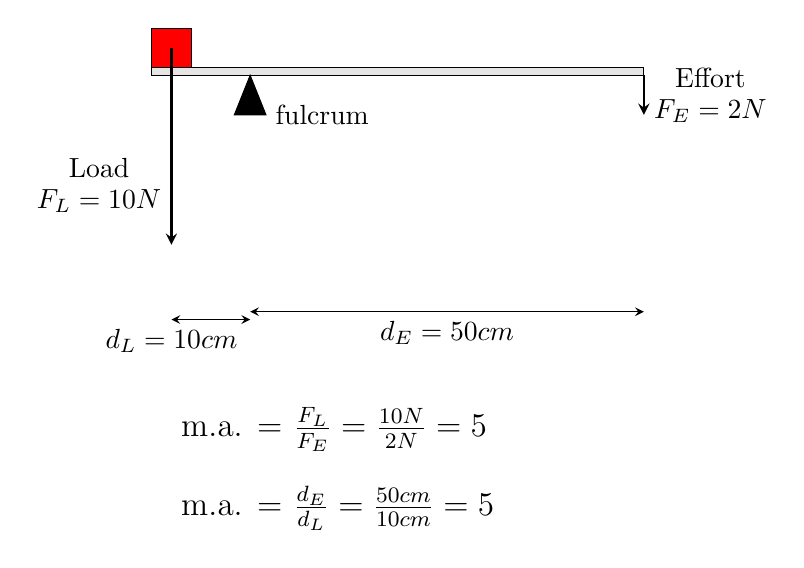
\begin{tikzpicture}[scale=1.0,>=stealth]
% First class lever

\draw[fill=gray!20] (-0.25,0) rectangle (6,0.1);
\draw[fill=black] (0.8,-0.5) -- (1.2,-0.5) node[right] {fulcrum} -- (1.0,0) -- cycle;

\draw[fill=red] (-0.25,0.1) rectangle (0.25,0.6);
\draw[->,thick] (0.0,0.35) -- (0.0,-2.15) node[midway,left,yshift=-0.5cm,align=center] {Load \\\\[-3ex] $F_L = 10N$};

\draw[->,thick] (6,0.0) -- (6,-0.5) node[midway,right,align=center] {Effort \\\\[-3ex] $F_E = 2N$};

% Distance markers
\draw[<->] (1,-3.0) -- (6,-3.0) node[midway,below,align=center] {$d_E= 50cm$};
\draw[<->] (0,-3.1) -- (1.0,-3.1) node[midway,below,xshift=-0.5cm,align=left] {$d_L = 10cm$};

% ma
\node[right] at (0,-4.5) {\large m.a. =  $\frac{F_L}{F_E}= \frac{10N}{2N} = 5$};
\node[right] at (0,-5.5) {\large m.a. =  $\frac{d_E}{d_L} = \frac{50cm}{10cm} = 5$};
\end{tikzpicture}

\end{document}